    %\setcounter{partie}{0} % Pour s'assurer que le compteur de \partie est à zéro dans les corrigés
    % \phantom{rrr}
    On considère la figure ci-dessous.

    \begin{enumerate}
        \item Démontrer que les triangles sont semblables.
        \item Calculer les longueurs $AC$ et $EF$.
    \end{enumerate}

    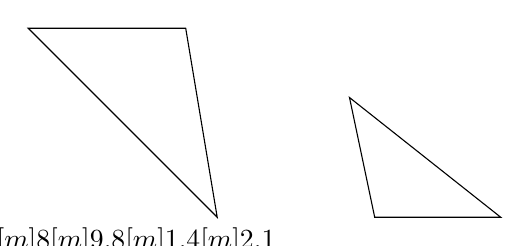
\begin{tikzpicture}[scale=0.4]
        % \quadrilageMailleCarree[black!30]{18}{8}
        % Points
        \coordinate (A) at (1,7);
        \coordinate (B) at (6,7);
        \coordinate (C) at (7,1);
        \coordinate (D) at (16,1);
        \coordinate (F) at (12,1);
        \coordinate (E) at (11.2,4.8);
        % Tracés
        \tkzLabelPoints[above](A,B,E);
        \tkzLabelPoints[below](C,F,D);
        \draw (A) -- (B) -- (C) -- cycle;
        \draw (E) -- (D) -- (F) -- cycle;
        \tkzLabelSegment[sloped,above](A,B){$\Lg[m]{8}$}
        \tkzLabelSegment[sloped,above](B,C){$\Lg[m]{9.8}$}
        \tkzLabelSegment[sloped](F,D){$\Lg[m]{1.4}$}
        \tkzLabelSegment[sloped,above](E,D){$\Lg[m]{2.1}$}
        \tkzMarkAngle[size=1,mark=|,mksize=2pt](C,A,B);
        \tkzMarkAngle[size=1,mark=|,mksize=2pt](E,D,F);
        \tkzMarkAngle[size=1,mark=o,mksize=2pt](B,C,A);
        \tkzMarkAngle[size=1,mark=o,mksize=2pt](F,E,D);
        \tkzMarkAngle[size=1,mark=||,mksize=2pt](A,B,C);
        \tkzMarkAngle[size=1,mark=||,mksize=2pt](D,F,E);
    \end{tikzpicture}


    {\color{red}
    \begin{enumerate}
        \item Puisque les triangles ont les trois mêmes angles alors ils sont semblables.
        \item Puisque les triangles sont semblables alors :

        $\dfrac{AB}{FD}=\dfrac{BC}{EF}=\dfrac{AC}{DE}$ donc $\dfrac{8}{\num{1.4}}=\dfrac{\num{9.8}}{EF}=\dfrac{AC}{\num{2.1}}$

        $\dfrac{8}{\num{1.4}}=\dfrac{AC}{\num{2.1}}$ donc $AC=\dfrac{8\times \num{2.1}}{\num{1.4}}=\Lg[m]{12}$

        $\dfrac{8}{\num{1.4}}=\dfrac{\num{9.8}}{EF}$ donc $EF=\dfrac{\num{9.8}\times \num{1.4}}{\num{8}}=\Lg[m]{1.715}$
    \end{enumerate}
    }
